\documentclass[numbering=fraction]{beamer}

\usepackage[utf8]{inputenc}
\usepackage[T1]{fontenc}
\usepackage[french]{babel}
\usepackage{blindtext}
\usepackage{tikzsymbols}
\usepackage{graphicx}
\usepackage{wrapfig}
\usepackage{bookman}
\usepackage{subcaption}
\usepackage[export]{adjustbox}


 % possibilité de démos
\usetheme[progressbar=frametitle]{metropolis}

%Define colors
\definecolor{wuppergreen}{RGB}{85, 171, 38}
\definecolor{background}{RGB}{255,255,255}

%Adding logo to title page
\titlegraphic{\raggedleft 
\includegraphics[width=3cm]{UNamur.png}}

%Adjust color theme
\setbeamercolor{frametitle}{bg=wuppergreen}
\setbeamercolor{title separator}{fg=wuppergreen}
\setbeamercolor{footline}{fg=gray}
\setbeamercolor{progress bar}{fg=black}

%Adding footer
\setbeamertemplate{frame footer}{\insertshortauthor~(\insertshortinstitute)}

\graphicspath{ {../Images/}}

%Set parameters for title page
\title{PIMS : Sprint Review 5}
\author[PIMS]{Luis Dierick \and Gaillard Matthys \and Bouncer Yassine \and Fundu Oliver \and Anderson Rosny \and Tom Marchal }
\institute{Université de Namur}
\date{\today}

\begin{document}

\begin{frame}[plain]{}
    \maketitle
\end{frame}

\begin{frame}{Table des matières}
    \tableofcontents
\end{frame}
\section{Rappel des événements de ce qu'il y a été fait}
\begin{frame}{Rappel}
    \begin{itemize}
        \item \textbf{Sprint 1} :
        \begin{itemize}
            \item Enquête de terrain : cellule TICE 
            \item Choix technologiques
        \end{itemize}
        \item \textbf{Sprint 2} : 
        \begin{itemize}
            \item Écriture de mockups et des scénarios en fonction des utilisateurds
        \end{itemize}
        \item \textbf{Sprint 3} :
        \begin{itemize}
            \item Début de la création de l'application
            \item Conception de la base de données.
        \end{itemize}
        \item \textbf{Sprint 4} :
        \begin{itemize}
            \item Création de la partie administration
            \item Gestion des rôles
        \end{itemize}
        \item \textbf{Sprint 5} :
        \begin{itemize}
            \item Intégration du rôle de superviseur.
            \item Gestion du processus d'inscription pour un étudiant.
        \end{itemize}
            
    \end{itemize}
\end{frame}
\section{Ce qui a été fait durant ce sprint}
\subsection{Burndown Chart}
\begin{frame}{Burndown chart}
    \centering
    
    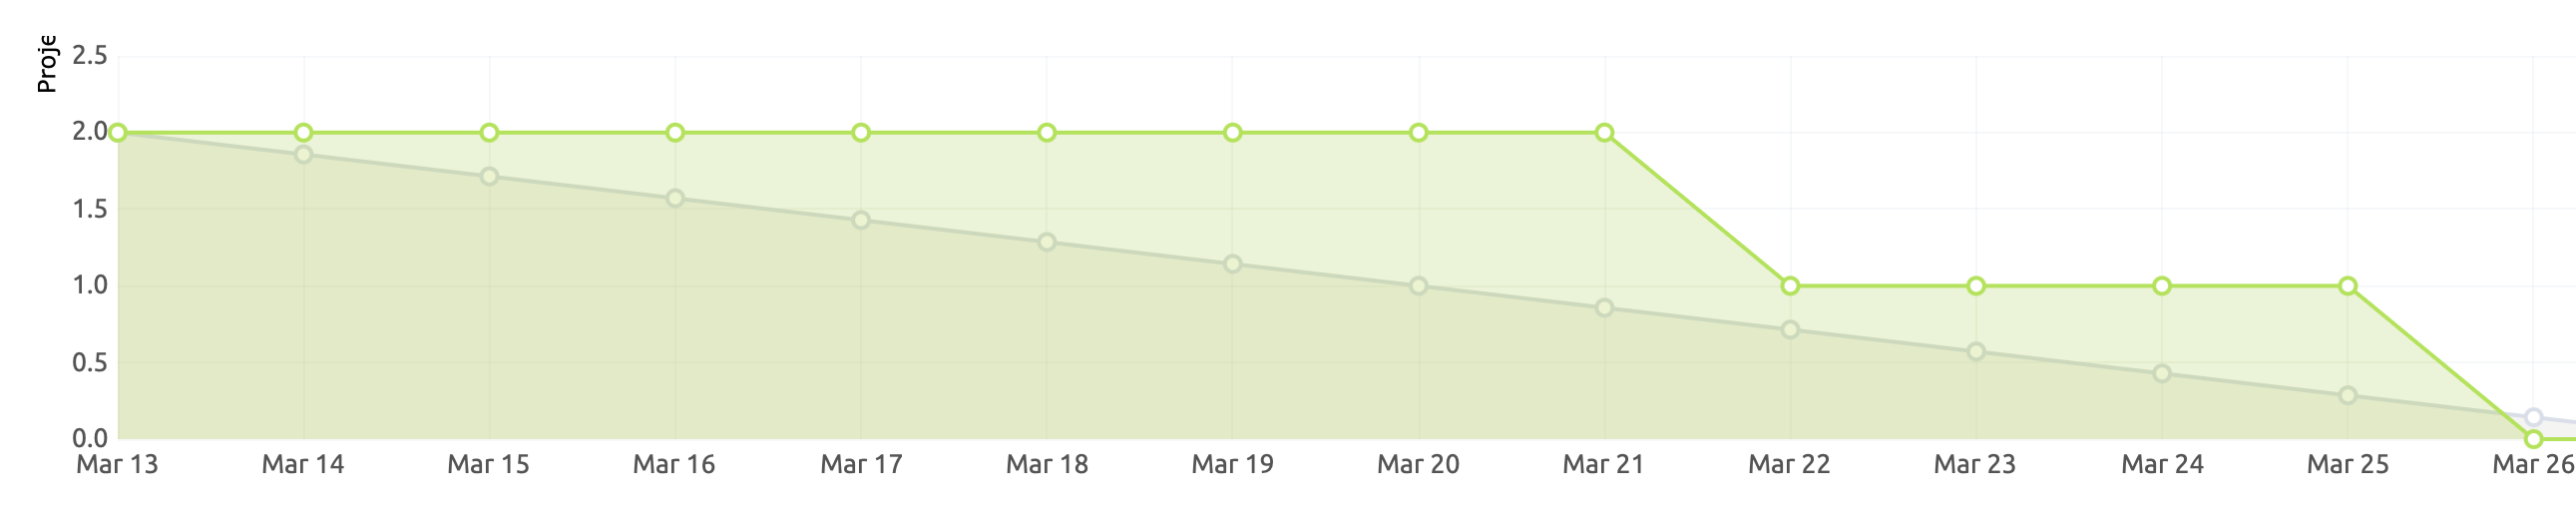
\includegraphics[width=1.1\textwidth]{burndownChart.png} 
\end{frame}
\subsection{Éléments faits}
\begin{frame}{Éléments faits}
   \begin{enumerate}
    \item Mettre le site web en ligne : dockerisation
    \item Ajout de la gestion des notes
    \item Gestion manuel de la vie d'un travail pour un professeur en charge d'un cours.
    \item Historique des sujets pour chaque cours.
    \item Archivage
    \item Diverses améliorations de l'interface graphique.
    \item Modifiction mineure de la BD.
   \end{enumerate}

\end{frame}
\section{Modifications}
\subsection{Modification de la BD}
\begin{frame}{Modification de la BD}
    \begin{enumerate}
        \item Ajout du système de note.
        \begin{itemize}
            \item Une note est associée à un travail.
            \item Une note globale est associée à un cours donc, au sujet.
        \end{itemize}
    \end{enumerate}
\end{frame}
\section{Scénarios}
\begin{frame}{Scénarios: illustration}
    \centering % Centrer le contenu
\vfill % Remplir l'espace vertical pour centrer verticalement
\textbf{\Large Démonstration} % Texte en gras et en grande taille
\vfill %
\end{frame}
\section{Travaux futurs et possibilité d'amélioration}
\begin{frame}{Travaux futurs et possibilité d'amélioration}
    \begin{itemize}
        \item Automatisation complète de la vie d'un travail.
        \begin{itemize}
            \item Utilisation d'un serveur redis pour la gestion des tâches asynchrones.
            \item Complémentarité avec celery.
            \item Possbilité de lancer des tâches en arrière plan en dehors du flux principal.
        \end{itemize}
        \item Ajout de nouveaux cours pour avoir une vue plus gobale des différents types travaux à réaliser
    \end{itemize}
    
\end{frame}

\end{document}